\setAuthor{Kaarel Kivisalu}
\setRound{piirkonnavoor}
\setYear{2022}
\setNumber{G 3}
\setDifficulty{3}
\setTopic{TODO}

\prob{Liumägi}
Liumägi koosneb kahest osast: kaldpind nurgaga $\alpha$ ja horisontaalne pind. Liumäe kõrgus on $h$ ja horisontaalne pikkus on $l$ (vt joonist). Liumägi tahetakse teha selline, et sealt alla lastes jõuaks täpselt liumäe lõppu, aga jäädes lõpus paigale. Võib eeldada, et üleminek kaldpinnalt horisontaalsele pinnale on sujuv. Milline peaks olema sellise liumäe jaoks hõõrdetegur $\mu$ liumäe ja allalaskja vahel?
\begin{figure}[h]
  \vspace{-1.5em}
  \centering
  {
    \tikzset{component/.style={draw,thick,circle,fill=white,minimum size=0.75cm,inner sep=0pt}}
    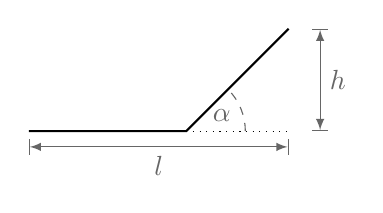
\begin{tikzpicture}
      %lines
      \draw[thick] (0,0) -- (2,0) -- (3.3,1.3);
      \draw[dotted] (2,0) -- (3.3,0);
      %angle
      \draw[dashed, black!60] (2.75,0) arc (0:45:.75);
      \draw[black!60] (2.45,0.2) node {$\alpha$};
      %lenghts
      \draw[|<->|, >=latex, black!60] (3.7,0)-- (3.7,1.3) node[midway, right]{$h$};
      \draw[|<->|, >=latex, black!60] (0,-0.2)-- (3.3,-0.2) node[midway, below]{$l$};
    \end{tikzpicture}
  }
  \vspace{-2em}
\end{figure}


\hint

\solu
\emph{Lahendus 1}:
Kalpinna pikkus on $h/\sin \alpha$ \p{0,5}. Horisontaalse pinna pikkus on $l-h/\tan \alpha$ \p{0,5}.
Hõõrdejõud kaldpinnast alla lastes on $F=\mu g \cos \alpha$ \p2. Energia jäävus (potentsiaalse energia muut on võrdne hõõrdejõu tööga):
\begin{equation*}
mgh = \mu mg \cos \alpha \cdot \frac{h}{\sin \alpha} + \mu mg \cdot \left(l- \frac{h}{\tan \alpha}\right). \quad \p4
\end{equation*}
Järelikult $\mu=h/l$ \p1.

\emph{Lahendus 2}:
Kiirendus kaldpinnast alla lastes on $a_1=g \sin \alpha - \mu g \cos \alpha$ \p2. Kalpinna pikkus on $h/\sin \alpha$ \p{0,5}. Järelikult kiirus kaldpinna lõpus on
\begin{equation*}
  v=\sqrt{\frac{2a_1h}{\sin \alpha}}. \quad \p{1,5}
\end{equation*}
Horisontaalse pinna pikkus on $l-h/\tan \alpha$ \p{0,5}. Kuna üleminek kaldpinnalt horisontaalsele pinnale on sujuv, siis kiirus ei muutu. Kiirendus horisontaalsel pinnal on $a_2= - \mu g $. Kuna liumäe lõpus peab alla lastes seisma jääma, siis
\begin{equation*}
  v=\sqrt{-2a_2\left(l-\frac{h}{\tan \alpha}\right)}.\quad \p{1,5}
\end{equation*}
Järelikult
\begin{equation*}
  2\mu g\left(l-\frac{h}{\tan \alpha}\right)=\frac{2h(g\sin \alpha - \mu g \cos \alpha)}{\sin \alpha}, \quad \p1
\end{equation*}
võrrantit lihtsustades saame, et $\mu=h/l$ \p1.
\probend